%%%%%%%%%%%%%%%%%%%%%%%%%%%%%%%%%%%%%%%%%
% Journal Article
% LaTeX Template
% Version 2.0 (February 7, 2023)
%
% This template originates from:
% https://www.LaTeXTemplates.com
%
% Author:
% Vel (vel@latextemplates.com)
%
% License:
% CC BY-NC-SA 4.0 (https://creativecommons.org/licenses/by-nc-sa/4.0/)
%
% NOTE: The bibliography needs to be compiled using the biber engine.
%
%%%%%%%%%%%%%%%%%%%%%%%%%%%%%%%%%%%%%%%%%

%----------------------------------------------------------------------------------------
%	PACKAGES AND OTHER DOCUMENT CONFIGURATIONS
%----------------------------------------------------------------------------------------

\documentclass[
	a4paper, % Paper size, use either a4paper or letterpaper
	10pt, % Default font size, can also use 11pt or 12pt, although this is not recommended
	unnumberedsections, % Comment to enable section numbering
	twoside, % Two side traditional mode where headers and footers change between odd and even pages, comment this option to make them fixed
]{LTJournalArticle}
\usepackage{amsmath}
\newcommand{\bra}[1]{\langle#1\rvert} % Bra
\newcommand{\ket}[1]{\lvert#1\rangle} % Ket
\newcommand{\qprod}[2]{ \langle #1 | #2 \rangle} %Inner Product
\newcommand{\braopket}[3]{\langle #1 | #2 | #3\rangle} % Matrix Element
\newcommand{\expect}[1]{ \langle #1 \rangle} % Expectation value

\addbibresource{sample.bib} % BibLaTeX bibliography file

\runninghead{An Intuitive Guide to QML} % A shortened article title to appear in the running head, leave this command empty for no running head

%\footertext{\textit{Journal of Biological Sampling} (2024) 12:533-684} % Text to appear in the footer, leave this command empty for no footer text

\setcounter{page}{1} % The page number of the first page, set this to a higher number if the article is to be part of an issue or larger work

%----------------------------------------------------------------------------------------
%	TITLE SECTION
%----------------------------------------------------------------------------------------

\title{An Intuitive Guide to Quantum Machine Learning\\ for the Classical Data Scientist} % Article title, use manual lines breaks (\\) to beautify the layout

% Authors are listed in a comma-separated list with superscript numbers indicating affiliations
% \thanks{} is used for any text that should be placed in a footnote on the first page, such as the corresponding author's email, journal acceptance dates, a copyright/license notice, keywords, etc
\author{%
	Amanda M Turney\textsuperscript{1}\thanks{Corresponding author: \href{mailto:amanda.marie.turney@gmail.com.com}{amanda.marie.turney@gmail.com}\\ \textbf{Received:} December 13, 2023}
}

% Affiliations are output in the \date{} command
\date{\footnotesize\textsuperscript{\textbf{1}}Luddy School of Informatics, Computing, and Engineering, Indiana University\\}


%----------------------------------------------------------------------------------------

\begin{document}

\maketitle % Output the title section

%----------------------------------------------------------------------------------------
%	ARTICLE CONTENTS
%----------------------------------------------------------------------------------------

\section{I. Motivation}

Impressive advances in the fields of data science and artificial intelligence have been made in the last few years by tools such as AlphaFold \autocite{jumper2021highly} 
for predicting 3D protein structure and ChatGPT \autocite{openai} for programming tasks, generating creative works, and answering questions, among many other applications. As technology 
continues to push the bounds of possibilities, a new force that has entered the data science field is quantum computing. While originally proposed back in the 1980s by Richard Feynman, 
quantum computing technology has matured immensely and a number of quantum companies have been started in the last decade \autocite{quantumhistory}. In the last two years, investments 
have grown substantially and in 2023 alone, both IBM and Atom Computing have announced 1000-qubit machines \autocite{atomcomputing, castelvecchiibm}. Combining these two technologies, 
quantum machine learning (QML) is an emerging field that researches the integration of quantum algorithms and machine learning.

While QML has had some success in the fields of chemistry and optimization, it is a difficult field to break into due to concepts such as entanglement and superposition which display 
quantum weirdness that is unintuitive to many people. There exist a plethora of online tutorials showing how to programmatically spin up quantum kernels or a quantum neural network, 
but an analysis of what makes these particular tools successful (especially compared to their classical counterparts) is often elusive. Thus, the aim of this paper is to provide an 
intuitive guide for readers with a background in data science to understand quantum machine learning and to illustrate how QML works in a fundamentally similar way to classical ML. 
The goal is to help eliminate some of the mystery of quantumness, to visually explain the power of quantum computing in machine learning tasks, and to discuss when and why to use 
quantum technologies for a given problem.

\section{II. Quantum Computing Basics Background}

\subsection{A. Qubits}
At the most fundamental level, the smallest piece of information that can be stored and processed by a quantum computer is a qubit. This is the quantum analog to a classical bit. 
Qubits can be implemented by a number of objects that behave quantumly such as electron orbitals of trapped ions, polarized photons, and spin-½ particles. Like classical bits, 
qubits can have two orthogonal states detonated by 0 and 1 and these can physically correspond to ground and excited orbitals, horizontal and vertical polarization, or up and down 
spins. However, qubits have the special feature that they are able to be in a superposition of both states. The qubits observable property (excitation, polarization orientation, or 
spin direction) is measured in the computational basis (usually along the z-axis) and always results in some binary result. But unlike classical bits which are always a predetermined 
0 or 1, qubits can have uncertainty in their measurement results. Specific quantum states are actually characterized by this uncertainty. For example, a quantum state can be defined 
as the following: 

\begin{equation}
	\psi =\alpha\ket{0} + \beta\ket{1}
	\label{eq:quantumstate}
\end{equation}

The coefficients above are called amplitudes and it is the square of these amplitudes that gives the probabilities of observing a $\ket{0}$ or $\ket{1}$ in the measurement. The 
last important aspect of these amplitudes is that they are complex numbers and thus can have a phase associated with them. This gives rise to the phenomenon of interference and 
happens when amplitudes are added together resulting in either constructive interference or destructive interference patterns. Clever quantum algorithms are ones that ensure that 
incorrect solutions are never measured at the end of a circuit because they are all canceled out through destructive interference, leaving only the correct solution(s) to be 
observed. Equation 1 represents a quantum state in the form known as the Dirac notation but quantum states are also often represented by vectors of length $2^n$ or matrices called 
density matrices of the shape $2^n$ x $2^n$, where $n$ is the number of qubits.

\subsection{B. Quantum Operators}
Just as classical computing has gates such as AND, OR, XOR, and NOT, there exists a set of quantum gates that can act on qubits. There are two different groups of gates: single 
qubit gates and multi-qubit gates. For example, just as the NOT gate acts on a single qubit and negates it, there exists an equivalent quantum operator called the Pauli-X gate. 
This gate rotates the qubit around the x-axis, resulting in a qubit that was initially in the $\ket{1}$ state to end in the $\ket{0}$ state and a qubit in the $\ket{0}$ state 
to end in the $\ket{1}$ state. The Pauli-X gate applies a full flip (180 degrees or pi radians) but qubits can be rotated around the y- and z-axis by any arbitrary number of degrees. 
One very important single gate operator is the Hadamard which first does a 90 degree rotation about the y-axis followed by a 180 degree rotation about the x-axis. The Hadamard is 
a crucial component to all quantum algorithms as it transforms qubits from the classical, computational basis to a superposition state. While the Pauli-X gate acting on the 
computational basis states ($\ket{0}$ and $\ket{1}$) is deterministic, the Hadamard introduces randomness where after the gate is applied to a $\ket{0}$ or $\ket{1}$ state, the new 
quantum state will now have a 50 percent chance of being measured in the $\ket{0}$ state and a 50 percent chance of being measured in the $\ket{1}$ state. An example of a 
multi-qubit gate is the controlled-NOT gate which requires two input qubits, a control and a target qubit, that flips the target qubit if the control qubit is in the $\ket{1}$ state. 
Other multi-qubit gates include controlled-Z gates and Toffoli gates.

One important rule that quantum operators always follow is that they are always reversible. Even though the Hadamard introduces some randomness into the state, there must exist an 
operator that can take that state of randomness and return it back to its initial state. This operator happens to also be the Hadamard, meaning it is its own inverse. Thus, when 
measuring quantum states, although things look classically random (where measurements cannot be predetermined and are only described by probabilities), it has a very definite state 
in the quantum world that a qubit can transition to and then transition back from. Lastly, while quantum operators can be implemented physically on quantum hardware, they are 
represented by Hermitian matrices.

\subsection{C. Special Phenomena}
The two main special phenomena that occur in the quantum world but not in the classical world are superposition and entanglement. Superposition was mentioned above where it was 
describing the ability of qubits to be in both state $\ket{0}$ and $\ket{1}$ simultaneously. It may be tempting to think of this state as a representation of knowledge of a system, 
meaning the qubit has some definite state but the observer simply does not know which and thus represents it probabilistically, just as a flipped coin has a 50 percent chance of 
heads and 50 percent chance of tails. However, this cannot be the correct interpretation because quantum states in superposition behave in a way that shows they must be both states 
at the same time. Otherwise, we would not see interference patterns and the canceling of certain possible events/measurements. The other special phenomena is called entanglement and 
describes the correlation between qubits. For example, two qubits can have the same state ($\ket{00}$ or $\ket{11}$) or they can have opposite states ($\ket{01}$ or $\ket{10}$). This 
property is shared between qubits and does not provide any information on the state of one of the single qubits in the pair and knowing that two qubits have the same state does not 
inform on whether the system is in state $\ket{00}$ or $\ket{11}$. An example of a gate that entangles two qubits is a controlled-NOT gate. Given a system with two qubits, one that 
is in state $ket{0}$ and the other in the equal superposition state defined below, 

\begin{equation}
	\psi =\frac{1}{\sqrt{2}}(\ket{0} + \ket{1})
	\label{eq:superposition}
\end{equation}

a controlled-NOT gate can use the qubit in superposition as the control and the qubit in state $\ket{0}$ as the target. Because the control qubit is both $\ket{0}$ and $\ket{1}$, it 
isn't known whether the target qubit gets flipped or not. If the control qubit is $\ket{0}$, then the target qubit stays in state $\ket{0}$ and thus the final state is $\ket{00}$. 
If the control qubit is $\ket{1}$, then the target qubit gets flipped and thus the final state is $\ket{11}$. If the system is measured, the only states that will ever be observed 
are $\ket{00}$ or $\ket{11}$ but prior to measuring, there is no way to determine which state it will be; all that is known is that the states will be the same. It is this coordination 
of measured results between qubits that seem inherently random that Einstein referred to as “spookiness at a distance” since qubits manage to always coordinate their respective behaviors 
no matter how far apart they are from each other.

\subsection{D. Quantum Algorithms}
In the classical world, computers manage bits (0 and 1) which are acted on by classical gates such as AND, XOR, and NOT. In the quantum world, quantum computers manage qubits which are 
acted on by quantum gates such as Hadamard and controlled-NOT. In the classical world, a series of gates can be put together in a defined procedure called an algorithm that is able to 
solve a specific problem. The same is true in the quantum computing world. However, there are only some specific problems for which a quantum algorithm can solve faster than a classical 
algorithm. Most everyday computations are quite efficient classically but a few notable exceptions are problems in cryptography and studying quantum systems such as chemical structures. 
Famous examples of algorithms that provide a quantum advantage include Deutch's algorithm, the Deutsch-Jozsa algorithm, the Bernstein-Vazirani problem, Simon's algorithm, Grover's 
algorithm, and Shor's algorithm. Quantum machine learning introduces algorithms that can be learned in order to solve new sets of problems and aims to use the power of quantum for a 
performance advantage or uncover solutions not reachable classically.

\section{III. QML Overview}
\subsection{A. Domains}
The field of quantum machine learning can be broken down into four areas of research depending on whether the data is classical or quantum and whether the algorithms are run on a classical 
computer or a quantum computer. This paper only covers the classical data and quantum algorithms area (CQ), which uses quantum algorithms to efficiently solve machine learning problems for 
classical datasets. However, the other three areas shown in Figure 1 are classical data and classical algorithms (CC) which focuses on quantum inspired classical algorithms, 
quantum data and classical computers (QC) which uses classical machine learning to assist in quantum computing tasks, and quantum data with quantum algorithms (QQ) which is very much in infancy.
Within CQ, much of this space focuses on quantum versions of many classical machine learning models. Supervised learning models include quantum variational algorithms \autocite{peruzzo2013variational} 
and quantum support vector machines \autocite{havlivcek2019supervised}. For unsupervised learning tasks, examples include the quantum PCA \autocite{lloyd2014quantum}, quantum clustering \autocite{aimeur2007quantum},
quantum variational autoencoders \autocite{khoshaman2018quantum}, and quantum generative adversarial networks \autocite{dallaire2018quantum}.

\begin{figure} % Single column figure
	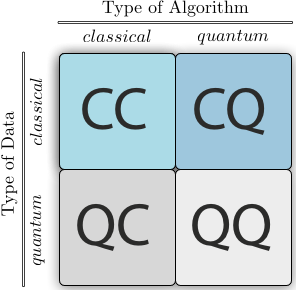
\includegraphics[width=\linewidth]{Qml_approaches.png}
	\caption{The four domains of quantum machine learning where the first letter indicates the type of data being processed and the second letter indicates the machine or alorithm that processes the data.}
	\label{fig:qmldomains}
\end{figure}

\subsection{B. Core Components of QML}
Regardless of the machine learning task, there are three core components that are part of every QML implementation. The first of which is the data encoding step. Just as data is encoded in 
binary on a classical computer, the data being processed must first be encoded and loaded onto a quantum computer in order to be processed by a quantum algorithm. One such method is called 
basis encoding. Given a quantum computer with N qubits, flipping each qubit to be $\ket{0}$ or $\ket{1}$ allows for the encoding of an N-bit binary string, i.e. 01011. Using the quantum 
property of superposition, multiple N-bit binary strings can be encoded at once. This method is used in many quantum algorithms such as Grover's, Shor's, and Deutsch-Jozsa where the input is 
a superposition of all values between 0 and $2^{n-1}$ such that the entire input space can be processed in parallel. Another encoding method is angle encoding, which rotates qubits by angles 
corresponding to data values. For example, given a data vector of N features, N qubits can be used to encode the datapoint by rotating each qubit by an angle determined by the $i^{th}$ value 
in the data vector. Unlike basis encoding, this method is used to only encode a single data point but that data point can now be a vector of floating point numbers instead of the binary string 
representation of a single integer. Lastly, arbitrary encoding is similar to angle encoding but is more efficient in its qubit utilization by encoding multiple parameter values onto a single 
qubit through rotations about different axes and the use of entanglement. Figure \ref{fig:dataencoding} shows an example of an arbitrary circuit, also known as a quantum feature map, that is 
used to encode 3 features on only 3 qubits.

\begin{figure} % Single column figure
	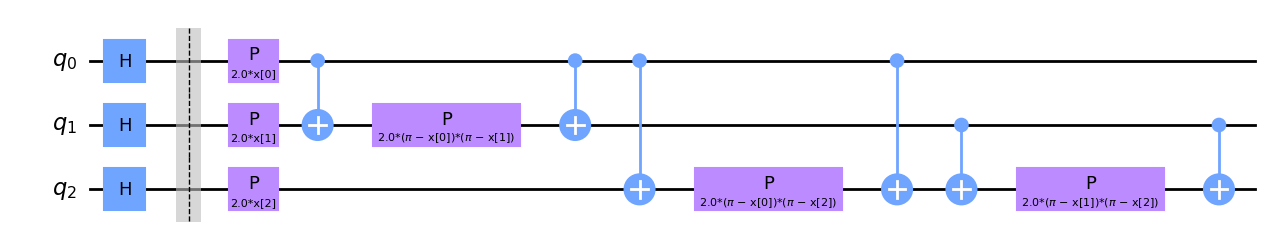
\includegraphics[width=\linewidth]{data_encoding.png}
	\caption{An example circuit showing arbitrary encoding of 12 features onto 3 qubits.}
	\label{fig:dataencoding}
\end{figure}

Another core component of quantum algorithms in QML are parameterized circuits, also known as variational forms or ansatzes. Once data is encoded in a quantum circuit, it must next be 
processed and transformed from its input state to some desirable output state. The variational form does this step and can be described as a template circuit consisting of rotation gates and 
entangling gates. However, the rotation angles for each gate are parameterized and the circuit must be trained in order to learn the optimal values of the variational form that best transform 
all inputs to their desired output quantum states. This is analogous to training a classical regression model for the parameters that best map the inputs to their target output values. 
However, note that while the quantum circuit performs the transformation of input state to an output state, it utilizes a classical computer to optimize those parameters using a cost function. 
Figure \ref{fig:ansatz} displays a variational form circuit with 18 trainable parameters, illustrating just one of many possible parameterized circuits. For example, rotational axes (y, z, or both), 
entangling gates (controlled-NOT, controlled-Z, etc.), and number of rotation and entangling layers are all choices that give rise to different variational forms. In selecting one variational 
form over another, the three major features that should be considered are expressibility, entangling capability, and hardware efficiency. Expressibility is the ability of the variational form 
to produce a quantum state that can reach nearly anywhere on the Bloch sphere, entangling capability is a measure of how entangled are the qubits of the circuit, and hardware efficiency 
refers to the reduction of errors through use of a limited set of quantum gates and optimal qubit connection topography \autocite{qiskitextbook2023}. High scores for all these features tends 
to result in better scoring quantum algorithms.

\begin{figure} % Single column figure
	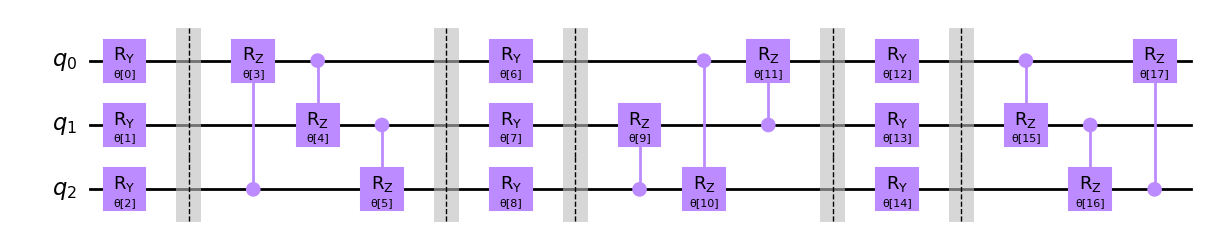
\includegraphics[width=\linewidth]{ansatz.png}
	\caption{An example circuit showing arbitrary encoding of 18 features onto 3 qubits.}
	\label{fig:ansatz}
\end{figure}

The last core component to any quantum algorithm in QML is the measurement step. Once data is encoded and processed, the individual qubits of the quantum circuit are measured where the qubit's 
observable property is read out, whether it be an orbital energy level, photon polarization orientation, or particle's spin direction. This measurement will correspond to either a $\ket{0}$ or 
a $\ket{1}$, but there are three main differences between quantum measurements and classical measurements. The first of which is that a quantum state's measurement result is probabilistic. 
Quantum circuits are usually run many times such that the measurement result samples can be used to estimate the underlying probabilistic distribution. This is very unlike classical bits which 
can be measured only once to know the state of either a 0 or 1. The second difference is that quantum states can be measured along different axes. Typically, qubits are measured along the 
computational basis which means that the observable property is projected onto the z-axis. For example, given a spin-½ particle, passing it through an inhomogeneous magnetic field oriented in 
the z-axis will cause particles to be deflected up or down within that axis, depending on their spin. But the particle could also be passed through a magnetic field oriented in the x-axis and 
could read out a spin direction within the x-axis. On the other hand, classical bits can only be measured on a single axis. The last and strangest difference between classical measurements and 
quantum measurements is that the act of measuring a qubit changes its state. When a quantum state is measured along a certain axis, it collapses to whatever state is measured. For instance, 
let's suppose there is a qubit that is in a quantum state defined by \ref{eq:superposition}. This qubit is measured (in the computational basis) and results in a $\ket{1}$. If this qubit is
measured again, it will again result in state $\ket{1}$. No matter how many times this qubit gets measured, it will never result in $\ket{0}$ because the original quantum state has collapsed. 
Any further computations with this qubit reveal that it acts exactly as a state $\ket{0}$ qubit and no longer behaves as both $\ket{0}$ and $\ket{1}$. However, another qubit can be prepared in 
the exact same way to be in the exact same quantum state as the initial qubit. But this qubit could instead result in a measurement read out of state $\ket{0}$. Thus, it is \emph{quantum states} that 
have measurements that are probabilistic each time, and not individual qubits. One other implication of this is that qubits cannot be measured along different axes, say both the x-axis and 
z-axis. Once a qubit is measured along one axis, its state has changed, so measuring the qubit along another is performing a measurement on the altered state and the result is no longer relevant 
to the original quantum state. Figure \ref{fig:qmlgencircuit} illustrates a general QML circuit containing the data encoding, data processing, and measurement components typically found in a QML algorithm.

\begin{figure} % Single column figure
	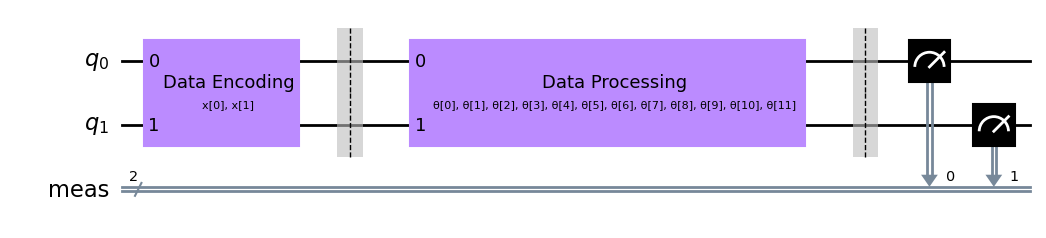
\includegraphics[width=\linewidth]{qml_general_circuit.png}
	\caption{A general QML circuit showing the data encoding step, data processing step, and measurements at the end of the circuit. However, this does not show any classical computations that
	often accompany QML such as classical optimization of parameters.}
	\label{fig:qmlgencircuit}
\end{figure}

\section{IV. Quantum Kernels}
Of all the possible quantum models listed in the section above, this paper takes a deep dive into quantum kernels because they are of particular interest for several reasons. The first of which 
is that they have demonstrated some of the most practical success and proven advantage compared to other quantum machine learning models \autocite{liu2021rigorous}. Studying these tools in 
particular should help in identifying and understanding what particular aspects of them contribute towards their success. The second reason is that Schuld makes an astute observation and 
demonstrates in \autocite{schuld2021supervised} that all supervised quantum machine learning models are actually quantum kernel methods. Therefore, if all quantum models can be rephrased as quantum kernel methods, 
then it makes sense to start an investigation of the quantum advantage there. The last reason for a deep dive into quantum kernels is that they most simply and plainly utilize quantum computers 
for their most essential feature: the Hilbert space. When comparing different types of successful quantum algorithms such as variational quantum algorithms versus Shor's and Grover's, there are 
some notable dissimilarities. For example, Shor's and Grover's have a solution-finding method built into their procedures that results in the correct solution(s) being measured at the end of 
the circuit, whereas variational quantum algorithms have no solution-finding process and instead rely on measurement readouts to go into a classical optimization function. However, what is 
common to all quantum algorithms is the casting of data to the high-dimensional Hilbert space where inner products can be efficiently calculated through measurements. This is exactly what 
quantum kernels do and the only thing that they do.

Now that the case for studying quantum kernels has been made, let's move on to describing them. In classical machine learning, it is common to map data to a higher dimensional space where 
hopefully patterns in the data are more obvious and easier to learn. Dealing with high dimensional data is often challenging though because storage and computations can be very resource intensive. 
However, many machine learning models are never actually concerned with the high dimensional data itself but rather, only the dot products of pairs of high dimensional data points. Thus, kernel 
functions are immensely useful as these functions are able to take as inputs the pair of data points in their original dimensions and compute the dot product of those two data points in the high 
dimensional feature space while only requiring the computational memory of the data in the original/low dimensional space.

\begin{equation}
	k(\vec{x_i}, \vec{x_j}) = \langle f(\vec{x_i}), f(\vec{x_j})\rangle
	\label{eq:kernel}
\end{equation}

Quantum computers are a perfect candidate for kernel functions because 1, they work in the high-dimensional Hilbert space, and 2, can compute dot products between two different quantum 
states very efficiently via measurements. The general procedure for computing a quantum kernel function is relatively straight forward and the high-level circuit diagram is shown in 
Figure \ref{fig:quantumkernel}. Given a quantum circuit with all qubits initialized to state 0 and two data points, the first step is to encode one of the data points using a quantum feature map (also known 
as arbitrary encoding). Next, the quantum state is then \emph{decoded} by the second data point. This decoding process is the same as the data encoding process but simply applies the series 
of gates of the quantum feature map in the reverse order, starting with the last gate applied first. The final step is to measure all the qubits at the end of the circuit. The actual value 
of the kernel function is the estimated probability, after repeating the circuit many times, of finding all qubits at the end of the circuit to be in state $\ket{0}$. As an example, 
let's consider two identical data points. The quantum feature maps for these two data points will be the same because they will have the same exact parameter values for all the rotation 
angles of the gates. Thus, with the quantum circuit starting with all qubits initialized in state $\ket{0}$, the data decoding phase of the circuit will simply undo the data encoding phase 
and the circuit will always revert back to its initial configuration of state $\ket{0}$ for all qubits. In general, data points that are highly similar should result in a final state of 
qubits all in the $\ket{0}$ state with a high probability whereas data points that are very dissimilar in the Hilbert space will rarely revert the circuit back to the initial configuration. 
What the circuit is actually doing is taking the dot product of two quantum states by measuring their transition amplitude. Once these distance/similarity values are calculated for all 
datapoint pairs within a dataset, this can be passed to classical machine learning models such as support vector machines.

\begin{figure} % Single column figure
	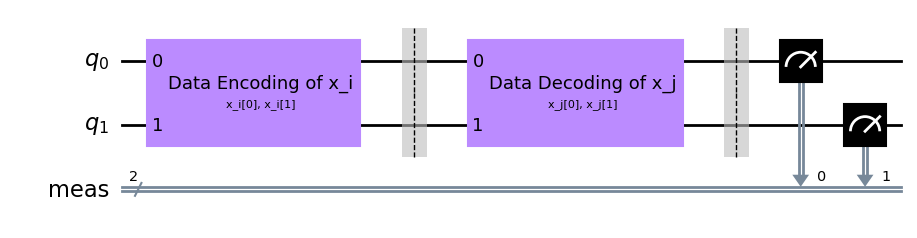
\includegraphics[width=\linewidth]{quantum_kernel.png}
	\caption{A general QML circuit performing the quantum kernel estimate. It first encodes for a datapoint $x_i$ using a quantum feature map, then it decodes
	by another data point, $x_j$, by running the respective quantum feature map in reverse. The circuit is run multiple times and the probability of measuring
	all $\ket{0}$ states at the end of the circuit is the kernel estimate.}
	\label{fig:quantumkernel}
\end{figure}

\section{V. Analysis of the Quantum Feature Space}
The inspiration for this paper comes from the work presented in \autocite{suzuki2020analysis} which analyzes feature maps for a quantum kernel based classifier. In this work, there are four 
datasets being investigated, which are named circles, moons, exponential, and xor and shown in Figure \ref{fig:datasets}. The two-dimensional data points have an assigned class label of either 
0 or 1 and the paper analyzes and compares the success of different quantum feature maps used in a quantum kernel based classifier model. The ultimate goal of the authors was to develop a 
method to compute, classically, a lower bound on the classifier accuracy score for each proposed quantum feature map for the purpose of screening a list of many potential feature maps. This 
would then give an idea of which feature map(s) would be best to actually test and run on quantum hardware for a particular problem dataset. The list of candidate feature maps the authors 
looked at are listed in Table \ref{tab:featuremaps} and the feature map circuit is shown in Figure \ref{fig:fm1}. However, while the practical goal of this paper was to develop a method by 
which to screen candidate feature maps, the most impactful piece was their work in representing and visualizing the quantum feature space. Despite focusing on the simple two qubit case, 
crucial insight was gained into what is behind the success of quantum algorithms.

\begin{figure}
	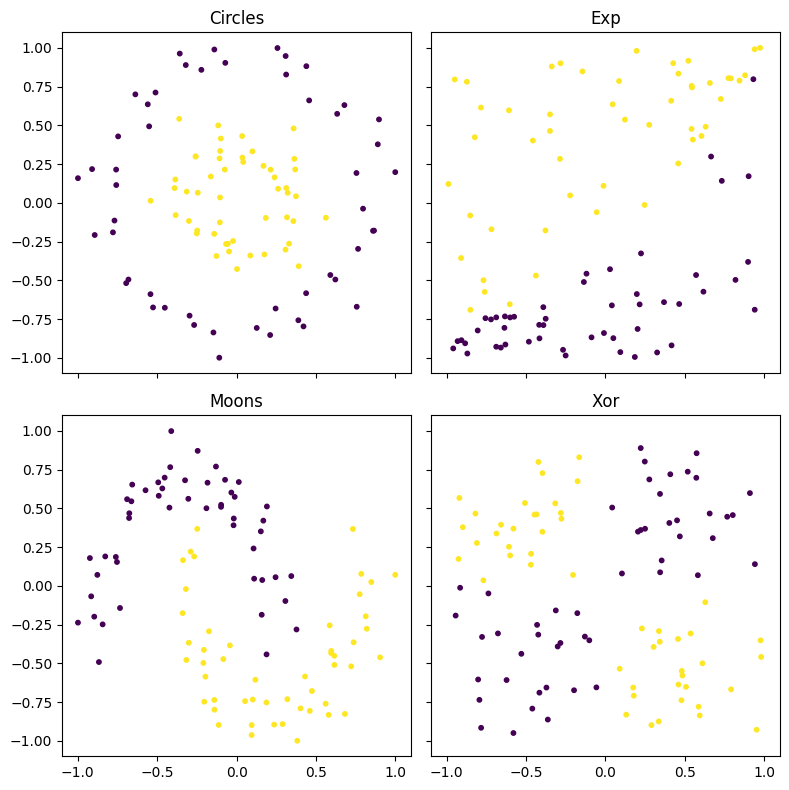
\includegraphics[width=\linewidth]{datasets.png}
	\caption{The toy datasets analyzed.}
	\label{fig:datasets}
\end{figure}

\begin{table} % Full width table (notice the starred environment)
	\caption{Feature maps analyzed.}
	\centering % Horizontally center the table
	\renewcommand{\arraystretch}{2}
	\begin{tabular}{L{0.12\linewidth} | L{0.05\linewidth} L{0.05\linewidth} R{0.35\linewidth}}
		Feature Map & $\phi_1(\vec{x})$ & $\phi_2(\vec{x})$ & $\phi_{1,2}(\vec{x})$ \\
		\midrule
		1 & $x_1$ & $x_2$ & $\pi x_1 x_2$ \\
		2 & $x_1$ & $x_2$ & $\frac{\pi}{2}(1-x_1)(1-x_2)$ \\
		3 & $x_1$ & $x_2$ & $exp(\frac{|x_1-x_2|^2}{8/ln(\pi)})$ \\
		4 & $x_1$ & $x_2$ & $\frac{\pi}{3cos(x_1)cos(x_2)}$ \\
		5 & $x_1$ & $x_2$ & $\pi cos(x_1)cos(x_2)$ \\
		\label{tab:featuremaps}
	\end{tabular}
\end{table}

\begin{figure}
	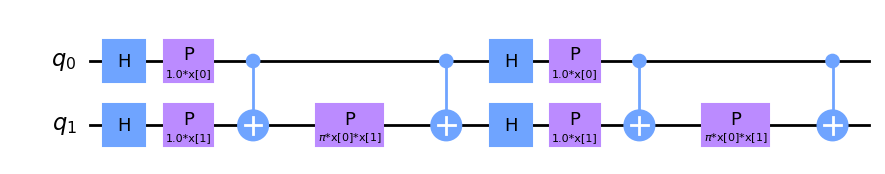
\includegraphics[width=\linewidth]{fm1.png}
	\caption{Quantum circuit for feature map 1 where $\phi(\vec{x})$ defines the two phase shift gate implemented on q1.}
	\label{fig:fm1}
\end{figure}

\subsection{A. Pauli Decomposition and Quantum Feature Space Visualizations}
The minimum training accuracy score that the authors compute in \autocite{suzuki2020analysis} requires first classically calculating the data encoded quantum states for each data point in the 
dataset. This quantum state is the result of encoding a given data point by a specific quantum feature map. These quantum states, represented in their density matrix form, are then expanded as 
a linear combination of basis states known as the Pauli operators. Just as the unit vectors along the x-, y-, and z-axes form the basis states of the $R^3$ space, the set of Pauli operators 
serve as the basis states for the vector space of $2^n$ x $2^n$ Hermitian matrices where n is the number of qubits. The set of Pauli operators for $n=1$ qubits are the three Pauli- X, Y, and 
Z gates plus the identity matrix $I$. For 2 qubits, there are 16 basis states which comes from the number of possible permutations of each of the two qubits getting one of the four possible 
Pauli operators applied to it. Given the label XX which represents applying Pauli-X gates to both qubits, we can describe the 16 basis states as II, IX, IY, IZ, XI, XX, XY, XZ, YI, YY, YX, YZ, 
ZI, ZX, ZY, and ZZ. Therefore, any density matrix (also sometimes called a density operator, although it describes a quantum state and not an operator) can be expressed as a linear combination 
of these 16 basis state operators. This process is called a Pauli decomposition and allows for the expression of a quantum state to be described by $4^n$ features.

Given an input domain, $x_1, x_2 \in [-1, 1]$, one can follow the above process to calculate the corresponding image of the quantum encoding function for each of the 16 dimensions. Colormaps 
for each feature map and each dimension were generated in \autocite{suzuki2020analysis} and were recreated and are shown in Figures \ref{fig:heatmap1} - \ref{fig:heatmap5}. Each colormap shows, 
in color, the value of the coefficient corresponding to the $x_1, x_2$ coordinate for a specific basis state and a particular feature map. The 16 plots for a specific feature map are then arranged 
in a 4 x 4 grid where the row and column position correspond to the basis state. The row number, $i$, and the column number, $j$, map to the basis state of the $i^{th}$ Pauli operator ({I, X, Y, Z}) 
applied to qubit 1 and the $j^{th}$ Pauli operator applied to qubit 2. For instance, row 2 and column 3 shows the colormap for XY. The quantum feature space is complex and not very intuitive to 
understand, which is why these plots are a great aid in visually understanding what the quantum feature space really looks like. Furthermore, \autocite{suzuki2020analysis} claims that the feature 
maps that produce patterns in these colormaps that look like the distributions of the problem dataset will have better accuracy scores. For example, the XY heatmap in Figure \ref{fig:heatmap1} 
looks very similar to the XOR dataset's distribution and the results of \autocite{suzuki2020analysis} do indeed show that this feature map performs best on the XOR dataset. This is a substantial 
claim because it elucidates how these quantum kernels are working and it ends up being a story that every data scientist knows very well. The observation that the best performing feature maps 
have shapes that look like the problem dataset is no different than trying to find a function that has the same shape as the problem dataset being modeled. For instance, fitting a line to linear 
data or an exponential to rapid growth data are examples of finding a function that has the same shape/pattern as the data. Therefore, although operating in a very high-dimensional space, quantum 
machine learning works fundamentally similar to classical machine learning.

\begin{figure}
	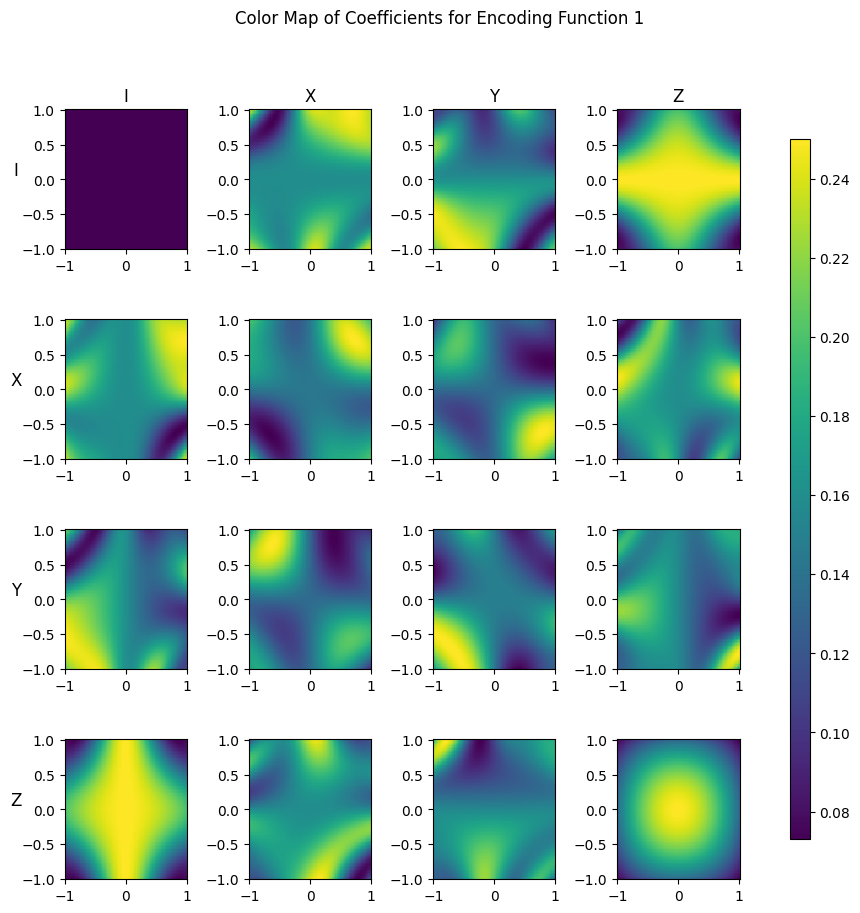
\includegraphics[width=\linewidth]{colormap_fm1.png}
	\caption{Colormaps for all 16 Pauli basis states for feature map 1, described in \ref{tab:featuremaps}.}
	\label{fig:heatmap1}
\end{figure}

\begin{figure}
	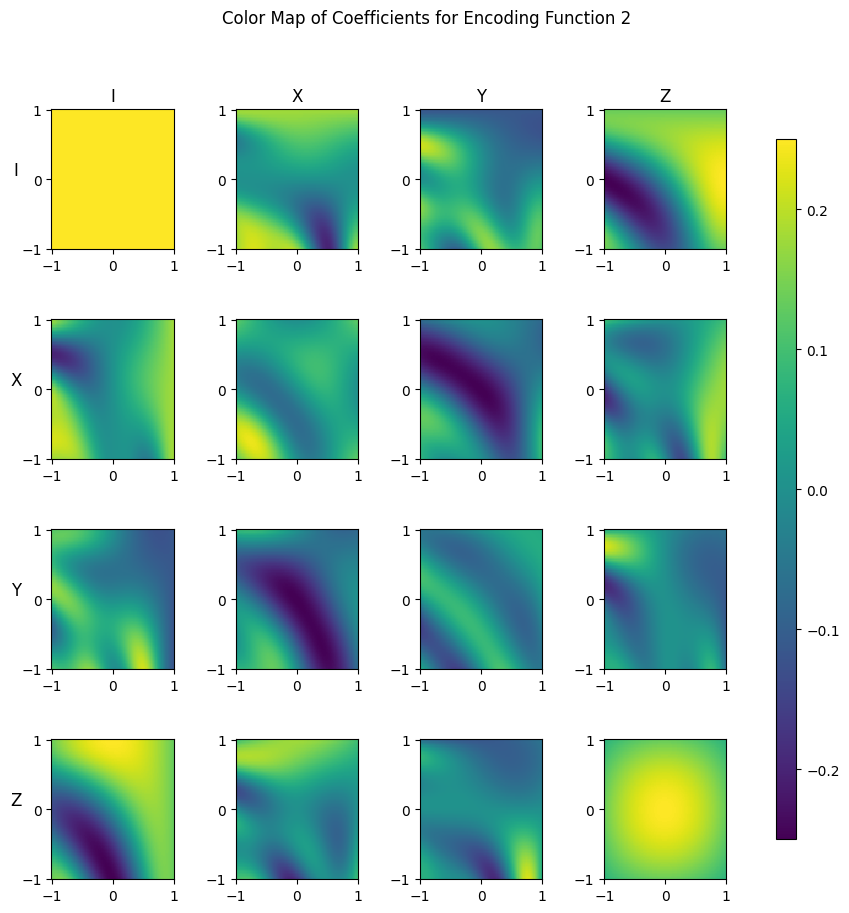
\includegraphics[width=\linewidth]{colormap_fm2.png}
	\caption{Colormaps for all 16 Pauli basis states for feature map 2, described in \ref{tab:featuremaps}.}
	\label{fig:heatmap2}
\end{figure}

\begin{figure}
	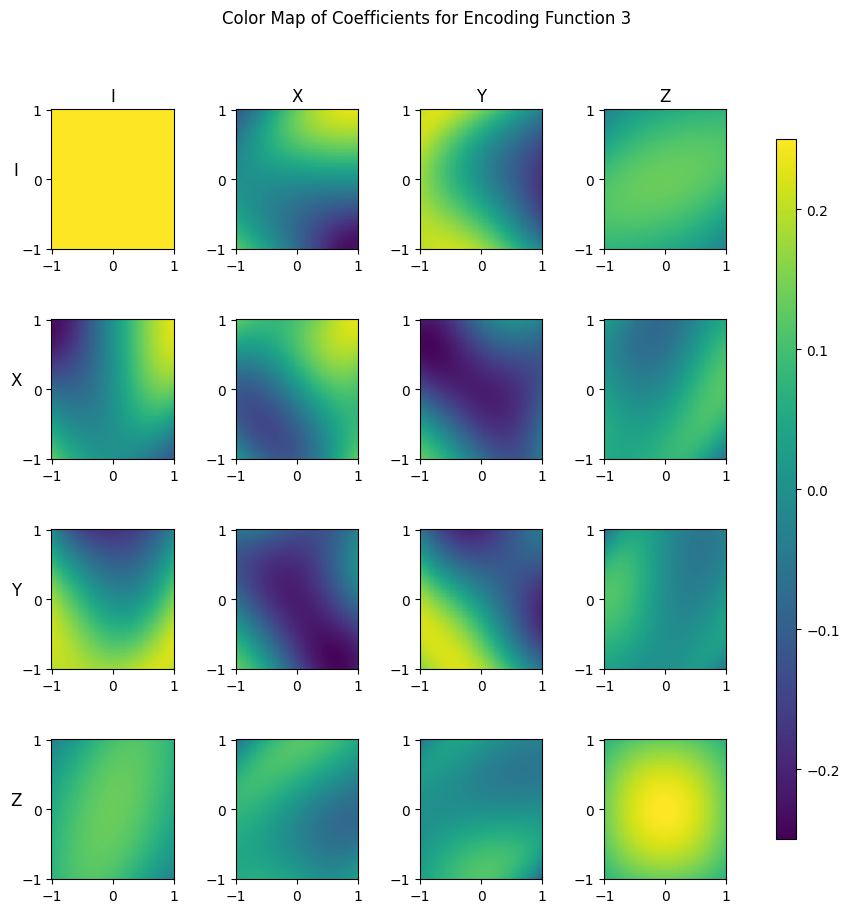
\includegraphics[width=\linewidth]{colormap_fm3.png}
	\caption{Colormaps for all 16 Pauli basis states for feature map 3, described in \ref{tab:featuremaps}.}
	\label{fig:heatmap3}
\end{figure}

\begin{figure}
	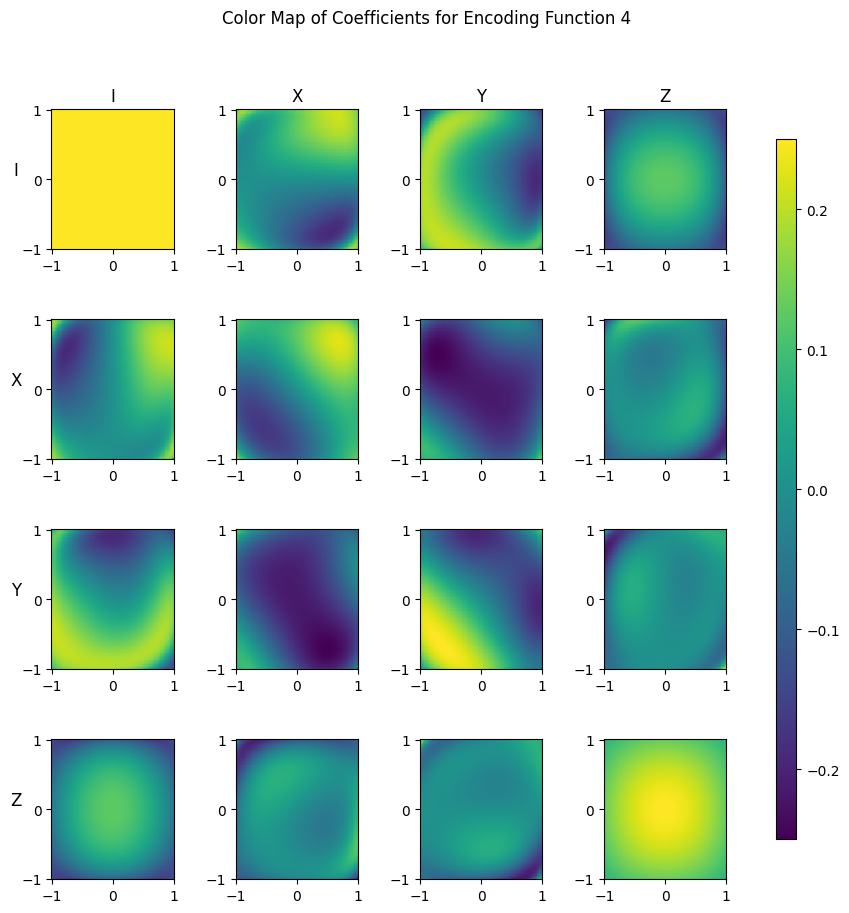
\includegraphics[width=\linewidth]{colormap_fm4.png}
	\caption{Colormaps for all 16 Pauli basis states for feature map 4, described in \ref{tab:featuremaps}.}
	\label{fig:heatmap4}
\end{figure}

\begin{figure}
	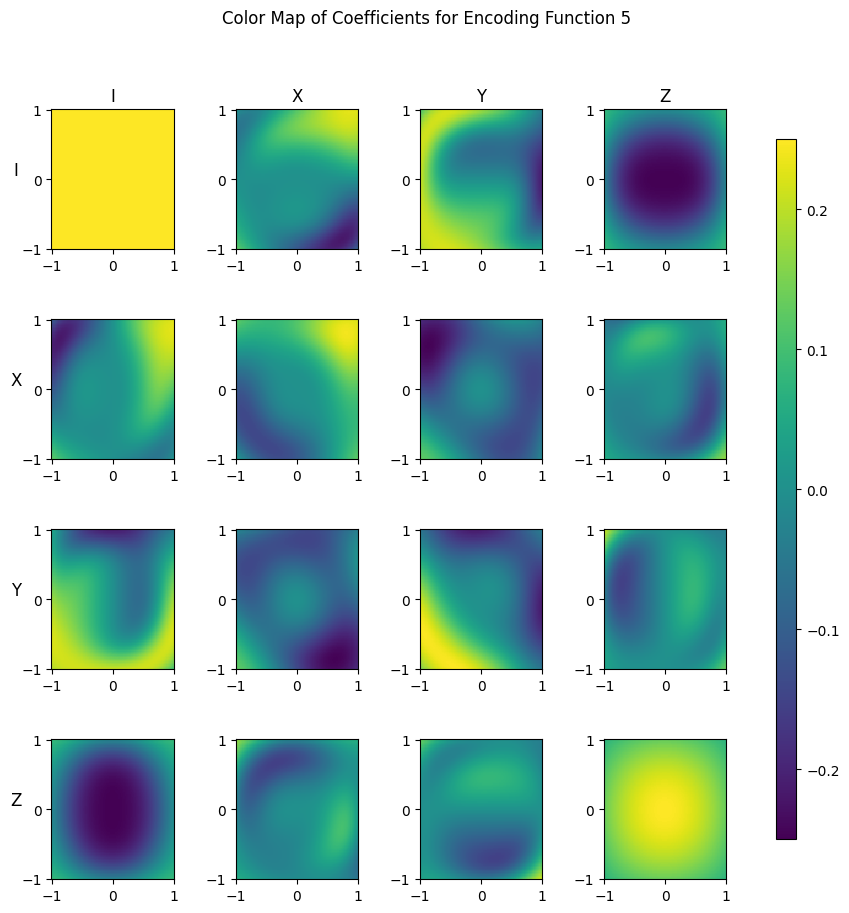
\includegraphics[width=\linewidth]{colormap_fm5.png}
	\caption{Colormaps for all 16 Pauli basis states for feature map 5, described in \ref{tab:featuremaps}.}
	\label{fig:heatmap5}
\end{figure}

\subsection{B. Minimum Training Accuracy}
While the colormaps described above are extremely illustrative in understanding quantum kernels, they are not a practice tool for screening feature maps because 1, they require many 
computations for the entire grid of $x_1, x_2 \in [-1, 1]$ and 2, they're qualitative nature makes them difficult to analyze. Therefore, the authors in \autocite{suzuki2020analysis} propose 
a minimum accuracy calculation that can aid in feature map screening for a given problem dataset. This method utilizes the 16-dimensional quantum dataset and applies a worse-case scenario, 
brute force method of estimating a minimum accuracy score that a classifier would achieve. This is done by first looking at the projections of the dataset on each of the 16 dimensions. For 
each axis, the objective is to find a boundary that best divides the data points along that axis such that all data points from class 0 fall to the left and all data points from class 1 fall 
to the right of the boundary. There are $N+1$ possible positions to place a hyperplane along the axis and all of which are tested and scored on how well they separate the data by their class 
label. The score of the most optimal hyperplane for that single axis is recorded and this is repeated for each of the 16 axes. Then, the highest score across all the axes is taken to be the 
minimum training accuracy score. Because this accuracy score is based on the ability to linearly separate the data by only a single axs rather than all 16, it represents a worse-case scenario 
of the classifier.

The minimum training accuracy computation method showed some success in being able to identify which quantum feature maps would have the most success in a quantum kernel based classifier.
\autocite{suzuki2020analysis} shows less than 100 percent training accuracy scores being achieved by the quantum-kernel based support vector machine (SVM) but my work in \autocite{myrepo} was 
unable to reproduce anything other than perfect accuracy for training scores. Considering a hard-margin SVM was used, it is hard to imagine why the authors were achieving less than perfect 
accuracy. Nonetheless, the minimum training accuracy scores (Table \ref{tab:minaccs}) generally align with the accuracy scores of the test datasets (Table \ref{tab:testaccs}). For example, 
the feature map with the best minimum training accuracy score achieved the highest test accuracy score for the exponential, moons, and xor datasets. A small extension of their work that I 
implemented was capturing which axis resulted that produced the minimum training accuracy score. This axis represents the best axis that was able to linearly separate the data. Results of this 
are shown in Table \ref{tab:bestaxes} and provide evidence to support the claim that quantum feature maps that produce shapes similar to the data distribution perform best. The most obvious 
support of this is the clear pick of the ZZ or ZI axis for the circles dataset. We also see a high frequency of feature map 1 selecting the YZ or ZY axes on the XOR dataset, which supports an 
observation made in an earlier section. However, as noted in \autocite{suzuki2020analysis}, classically computing the coefficients of the quantum states for the entire dataset is not generally 
feasible as the number of dimensions of the quantum feature space grows exponentially with the number of qubits. Their work represents a proof-of-concept for the methodology whereas the next 
section looks at extending this work for more efficient ways to screen candidate feature maps.

\begin{table} % Full width table (notice the starred environment)
	\caption{The average minimum training accuarcies computed using the method proposed by \autocite{suzuki2020analysis} across 30 cross-fold validations.
	}
	\centering % Horizontally center the table
	\renewcommand{\arraystretch}{2}
	\begin{tabular}{L{0.12\linewidth} | L{0.15\linewidth} L{0.15\linewidth} R{0.15\linewidth} R{0.15\linewidth}}
		Feature Map & Circles & Exp & Moons & XOR \\
		\midrule
		1 & 100\% & 84.8\% & 84.8\% & 96.8\%\\
		2 & 100\% & 85.5\% & 84.5\% & 92.7\% \\
		3 & 100\% & 95.0\% & 89.5\% & 89.8\%\\
		4 & 100\% & 89.8\% & 89.8\% & 86.2\%\\
		5 & 100\% & 88.0\% & 90.0\% & 87.8\%\\
		\label{tab:minaccs}
	\end{tabular}
\end{table}

\begin{table} % Full width table (notice the starred environment)
	\caption{The average test accuracy scores for 30 cross-fold validations.
	}
	\centering % Horizontally center the table
	\renewcommand{\arraystretch}{2}
	\begin{tabular}{L{0.12\linewidth} | L{0.15\linewidth} L{0.15\linewidth} R{0.15\linewidth} R{0.15\linewidth}}
		Feature Map & Circles & Exp & Moons & XOR \\
		\midrule
		1 & 93.8\% & 78.7\% & 68.3\% & 93.0\%\\
		2 & 87.2\% & 79.0\% & 83.0\% & 84.8\% \\
		3 & 97.0\% & 89.3\% & 70.0\% & 91.2\%\\
		4 & 97.3\% & 85.3\% & 85.3\% & 87.2\%\\
		5 & 97.3\% & 83.5\% & 88.3\% & 85.7\%\\
		\label{tab:testaccs}
	\end{tabular}
\end{table}

\begin{table*} % Full width table (notice the starred environment)
	\caption{The top 3 axes most frequently chosen as best axis to linearly separate data in 
	minimum training accuracy calculation across 30 cross fold validations are shown in the 
	table. This provides evidence to the claims made in \autocite{suzuki2020analysis} that feature
	maps that have patterns in the feature space resembling the data distribution results in the
	best accuracy.
	}
	\centering % Horizontally center the table
	\renewcommand{\arraystretch}{2}
	\begin{tabular}{L{0.12\linewidth} | L{0.2\linewidth} L{0.2\linewidth} R{0.2\linewidth} R{0.2\linewidth}}
		Feature Map & Circles & Exponential & Moons & XOR \\
		\midrule
		1 & ZZ(20), IZ(6), ZI(4) & YI(8), ZY(7), IY(3) & IX(8), IY(8), YZ(7) & YX(26), XY(3), YI(1)\\
		2 & ZZ(30) & IY(8), YI(5), IX(4) & XI(14), YI(6), XZ(5) & YZ(6), IX(6), YX(5) \\
		3 & ZZ(21), ZI(5), IZ(3) & ZX(19), YZ(6), IY(4) & XI(12), XZ(6), IY(5) & YX(11), XY(6), ZI(5)\\
		4 & ZI(29), IZ(1) & IY(21), XI(5), YI(1) & XI(18), IY(7), ZY(4) & YX(13), XY(7), XI(5)\\
		5 & ZI(29), IZ(1) & IY(7), ZX(6), XI(6) & IY(9), ZX(8), XZ(4) & YX(15), XY(7), IX(3)\\
		\label{tab:bestaxes}
	\end{tabular}
\end{table*}

\section{VI. Efficient Quantum Kernel Screening}
\subsection{A. Random Feature Selection}
The most computationally intensive part of the minimum training accuracy score is the requirement of computing the coefficients for all 16 axes for the entire dataset. A more efficient screening 
technique will not require each dimension for each datapoint to be computed and therefore, this paper looks at two methods of reducing the number of computations. The first of which is random 
selection and attempts to estimate the minimum accuracy by randomly selecting a subset of the 16 Pauli axes for batches of data. Due to the small dataset size (100 in total with each cross-fold 
validation using only 20 data points), there is a limitation in the number of options for batch size. To ensure equal batch sizes, batches of 4 or 10 could be selected resulting in 5 or 2 batches 
to process respectively. I selected a batch size of 10 data points which leaves only 2 batches per cross-fold validation to be processed but ensures that each batch has enough data points to 
reveal the most prominent features of the underlying data distributions. Within each batch, the method randomly selects 5 axes from the 16 to test. With only two batches of data per cross-fold 
validation, a larger number of axes to random select was chosen. However, this parameter can be tweaked and might depend on the dataset size. For a larger dataset with more batches, a smaller 
subset of axes could be sampled. This method looks similar to the original method but computes the accuracy for only the subset of axes for each batch and reports the best accuracy found. The 
results of the random selection feature method are shown in Table \ref{tab:rsresults} and the number of Pauli decomposition axis evaluations are reported in Table \ref{tab:rsevals}. The number of evaluations is uniform across 
each feature map and dataset due to the static number of axes and batches being processed. The total number of Pauli decomposition axis evaluations performed by the random feature selection 
method requires only 31.25\% of the computations required by the original method which is a decent improvement. The other advantage of this method is that the number of computations is uniform 
and thus the scaling of this method can be easily predicted. However, this method doesn't quite reveal the divergences in skill across the feature maps that we would expect compared to the actual 
computed minimum accuracy scores. We do see in Table \ref{tab:rsresults} that feature map 1 performs best on the XOR dataset and that encoding feature 3 scores highest for the exponential dataset 
but overall, the best scores are only marginally higher than the next best feature maps compared to the clear winning scores seen in the original method. We also do not see the same feature map 
performing the best for the moons dataset but the actual minimum accuracy scores for multiple feature maps are all very close to each other in this case.

\begin{table} % Full width table (notice the starred environment)
	\caption{The average estimated minimum training accuarcy scores calculated by the Random Selection method across 30 cross-fold validations.
	}
	\centering % Horizontally center the table
	\renewcommand{\arraystretch}{2}
	\begin{tabular}{L{0.12\linewidth} | L{0.15\linewidth} L{0.15\linewidth} R{0.15\linewidth} R{0.15\linewidth}}
		Feature Map & Circles & Exp & Moons & XOR \\
		\midrule
		1 & 98.0\% & 91.0\% & 89.0\% & 96.7\%\\
		2 & 96.0\% & 91.3\% & 90.7\% & 95.3\%\\
		3 & 98.7\% & 95.3\% & 95.3\% & 93.0\%\\
		4 & 99.7\% & 91.7\% & 91.2\% & 91.0\%\\
		5 & 100.0\% & 94.0\% & 93.3\% & 92.7\%\\
		\label{tab:rsresults}
	\end{tabular}
\end{table}

\begin{table} % Full width table (notice the starred environment)
	\caption{The average number of Pauli decomposition axis computation evaluations required by the Random Selection method across 30 cross-fold validations.
	}
	\centering % Horizontally center the table
	\renewcommand{\arraystretch}{2}
	\begin{tabular}{L{0.12\linewidth} | L{0.15\linewidth} L{0.15\linewidth} R{0.15\linewidth} R{0.15\linewidth}}
		Feature Map & Circles & Exp & Moons & XOR \\
		\midrule
		1 & 100 & 100 & 100 & 100\\
		2 & 100 & 100 & 100 & 100\\
		3 & 100 & 100 & 100 & 100\\
		4 & 100 & 100 & 100 & 100\\
		5 & 100 & 100 & 100 & 100\\
		\label{tab:rsevals}
	\end{tabular}
\end{table}

\subsection{B. Adaptive Feature Selection}
The next proposed method is designed to use computation resources in a smarter way by implementing an adaptive feature selection process. This method processes the data in pairs of balanced 
data points (one from class 0 and one from class 1). Starting with 4 data points, it computes the accuracies of the best hyperplane along each of the 16 Pauli axes and then selects the 
best subset of axes. Then, it will process the next two data points and compute the accuracies of those 6 data points along the subset of previously selected Pauli axes. It keeps repeating 
this, processing more pairs of data points, but on a shrinking subset of Pauli axes until some stopping criteria is met. The stopping criteria involves some minimum number of data points 
being evaluated to provide a good enough estimate of the minimum accuracy score. Sometimes, only one axis will remain by this stopping point and the best accuracy of this single axis is 
reported; other times, there will be multiple axes still in play but they have comparable accuracies and the maximum is selected and reported out. Therefore, axes that are clearly poor 
fits of the data are dropped early in the process and only the best performing axes are calculated for the following batches of data.

The selection of the best subset of Pauli axes that is done on each iteration as described above is determined by looking at the mean and standard deviation of the accuracy scores achieved by 
each of the Pauli axes being processed. For instance, on the first iteration looking at 4 data points and computing accuracies for all 16 axes, the mean and standard deviations of the 16 
accuracies achieved by the optimal hyperplane on each dimension are calculated. An adaptive cutoff is set based on some number of standard deviations below the mean accuracy score and all 
axes that perform better than that cutoff continue on for future iterations. The rate of which the axes discarded at each iteration can be controlled by two parameters: adaptive rate and 
initial standard deviations. The adaptive rate controls the exponential rate by which the number of standard deviations below the mean shrinks on each iteration and the initial standard 
deviations parameter is the initial number of standard deviations and determines how aggressive to cut on the first iteration.

The estimated minimum accuracy scores from this method are shown in Table \ref{tab:asresults} and the performance results, measured in number of Pauli decomposition evaluations, is shown in 
Table \ref{tab:asevals}. Overall, the number of Pauli evaluations dropped to 27.9\% of the number required by the original method which is comparable to the random selection method, allowing for
a fair comparison between these two methods considering they used similar computational resources. While the random selection had uniform computation for each feature map and dataset, the 
adaptive selection approach dynamically allocates more computations when needed. For instance, in Table \ref{tab:asevals}, we see that the feature map 1 for the moons dataset only used an 
average of 81.6 Pauli axis evaluations whereas encoding function 5 in the circles dataset required 25\% more Pauli axis evaluations. Overall, the circles dataset required the most evaluations 
despite being the easiest dataset for the feature maps to classify. While this was't initially intuitive, it was found that this was the case because there were multiple axes performing equally 
well and the adaptive selection algorithm was unable to drop as many axes off at each iteration. Without a clear winner early on, a handful of axes end up getting processed all the way until 
the stopping criteria is met. Therefore, this method operates as intended in using the necessary resources for each use case to determine the best estimate possible. Looking at Table 
\ref{tab:asresults}, we can also see that the estimated minimum training accuracy scores this method computes are much closer to the original values computed compared to the random selection 
method. For example, it finds a minimum score of 100\% for all feature maps on the circles dataset which is the same as the original method. It also clearly identifies feature map 1 as the most 
suitable for the XOR dataset and feature map 3 for the exponential dataset, both scoring accuracies that are very close to the original values computed. Overall, this method worked well in 
efficiently predicting which feature map would have the best training accuracy on a dataset at a fraction of the resources required by the original method. The downside of this method though 
is that the number of computations, having a dynamic nature, cannot be easily estimated when assessing how this method would scale.

\begin{table} % Full width table (notice the starred environment)
	\caption{The average estimated minimum training accuarcy scores calculated by the Adaptive Selection method across 30 cross-fold validations.
	}
	\centering % Horizontally center the table
	\renewcommand{\arraystretch}{2}
	\begin{tabular}{L{0.12\linewidth} | L{0.15\linewidth} L{0.15\linewidth} R{0.15\linewidth} R{0.15\linewidth}}
		Feature Map & Circles & Exp & Moons & XOR \\
		\midrule
		1 & 100.0\% & 86.1\% & 88.9\% & 97.8\%\\
		2 & 100.0\% & 87.5\% & 88.3\% & 93.1\%\\
		3 & 100.0\% & 95.0\% & 93.3\% & 914\%\\
		4 & 100.0\% & 89.2\% & 93.3\% & 87.8\%\\
		5 & 100.0\% & 87.8\% & 93.1\% & 86.7\%\\
		\label{tab:asresults}
	\end{tabular}
\end{table}

\begin{table} % Full width table (notice the starred environment)
	\caption{The average number of Pauli decomposition axis computation evaluations required by the Adaptive Selection method across 30 cross-fold validations.
	}
	\centering % Horizontally center the table
	\renewcommand{\arraystretch}{2}
	\begin{tabular}{L{0.12\linewidth} | L{0.15\linewidth} L{0.15\linewidth} R{0.15\linewidth} R{0.15\linewidth}}
		Feature Map & Circles & Exp & Moons & XOR \\
		\midrule
		1 & 92.00 & 88.13 & 81.60 & 88.13\\
		2 & 85.93 & 84.67 & 87.20 & 89.40\\
		3 & 95.93 & 93.60 & 90.67 & 84.80\\
		4 & 101.20 & 88.33 & 82.87 & 86.86\\
		5 & 101.40 & 90.27 & 87.93 & 85.40\\
		\label{tab:asevals}
	\end{tabular}
\end{table}

\section{VII. Discussion and Conclusion}
In section VA, sets of 16 heatmaps illustrate the quantum feature space for all five feature map studied and extension on work done by other authors show that datasets are classified more easily 
when the quantum kernel based classifier models use a feature map that posses similar patterns. This paper identified the exact Pauli axes that best linearly separate the data which allowed for 
the drawing of connection between quantum machine learning and classical machine learning. That is, a feature map that models our data well in the high-dimensional Hilbert space is able to perform 
better for classification. Thus, identifying the most ideal feature map through either candidate screening or kernel alignment (not discussed in this paper) involves finding a quantum function 
that best fits a given dataset. While it is comforting to see this familiar machine learning task apply to QML, it also naturally raises the question of whether QML has the same challenges as 
ML in these tasks. For instance, in variational quantum algorithms, the problem of barren plateaus also exist.

There is an inherit advantage for QML by having access to the Hilbert space and allowing for efficient computations in this high-dimiension space. But does the quantum advantage exist partially 
due to a larger collection of quantum functions to select from compared to classical functions? Or does a quantum advantage come from the ability to find these quantum functions that model a 
problem dataset more efficiently than classical algorithms are able to find functions that best fit data? QML only has a potential at outperforming classical ML when functions are difficult to 
compute classically but are natural quantumly. But in those cases when QML does outperform classical ML, there isn't a clear explanation as to where the performance gain comes from. 

In evaluating when and where to use quantum technology for a machine learning task, there are a few aspects to consider. One of which is quantum algorithms are a natural fit for studying quantum 
systems and some optimization problems that can be casted to Hamiltonians. However, quantum computers have a limitation in their ability to process big data. Data encoding tends to be a very 
inefficient step and with only a relatively small number of qubits that can be used with some limitation in the connection topography that can lead to decoupling and noise, quantum computers 
currently do best solving high compute but low data size problems. Therefore, it is the opinion of the reader that in the current state of knowledge, there is a fair balance between the advantages 
and disadvantages to quantum machine learning that make it not a clear winning technology in general. Instead, there is expected to specific use cases for which it will perform well and hopefully 
future research on the performance advantage can inspire new classical algorithms as well as identify more use cases for quantum computing with focus on how to map these as quantum problems. 
%----------------------------------------------------------------------------------------
%	 REFERENCES
%----------------------------------------------------------------------------------------

\printbibliography % Output the bibliograph
%----------------------------------------------------------------------------------------

\end{document}
